\documentclass[11pt, handout]{beamer} % To remove reveals for printing.
%\documentclass[12pt]{beamer}


\usepackage{color}
\usefonttheme{professionalfonts} % using non standard fonts for beamer
\usefonttheme{serif} % default family is serif
%\usepackage{fontspec}
%\setmainfont{Liberation Serif}
\definecolor{blank}{gray}{1} %1 to hide


\graphicspath{{.}{Figures/}}
\usetheme{boxes}
\def\b{$\bullet $}
\def\ds{\displaystyle}
\def\BE{\mathbb{E}}
\def\Var{\mathbb{V}\mbox{ar}}
\def\cov{\mathbb{C}\mbox{ov}}
\def\cor{\mathbb{C}\mbox{or}}


\newcommand\hideit[1]{%
  \only<0| handout:1>{\mbox{}}%
  \invisible<0| handout:1>{#1}}

\newcommand{\e}{\varepsilon}
\newcommand{\al}{\alpha}
\newcommand{\s}{\sum_{i=1}^n}
\newcommand{\shat}{\hat{\sigma}^2}
\newcommand{\bhat}{\hat{\bbeta}}
\newcommand{\ahat}{\hat{\alpha}}
\newcommand{\be}{\mbox{\boldmath{$\varepsilon$}}\unboldmath}
\newcommand{\rd}{\mathrm{d}}
% Standardized forms for name of S-plus
\renewcommand{\S}{S-P{\footnotesize LUS }}
\newcommand{\Shead}{S-P{\normalsize LUS}}
\newcommand{\lreg}{\begin{equation}y_i=\alpha+\beta x_i +\e_i,\end{equation}}
\newcommand{\bx}{\mbox{$\mathbf{x}$}}
\newcommand{\bz}{\mbox{$\mathbf{z}$}}
\newcommand{\xvec}{\mbox{$\bx_1,\ldots,\bx_n$}}
\newcommand{\yxvec}{\mbox{$y_1=\eta(\bx_1),\ldots,y_n=\eta(\bx_n)$}}
\newcommand{\by}{\mbox{$\mathbf{y}$}}
\newcommand{\bh}{\mbox{$\mathbf{h}$}}
\newcommand{\bt}{\mbox{$\mathbf{t}$}}
\newcommand{\bbeta}{\mbox{\boldmath{$\beta$}}\unboldmath}
\newcommand{\bdelta}{\mbox{\boldmath{$\delta$}}\unboldmath}
\newcommand{\btheta}{\mbox{\boldmath{$\theta$}}\unboldmath}
\newcommand{\bo}[1]{\mbox{$\mathbf{#1}$}}
\newcommand{\yxpvec}{\mbox{$y_1'=\eta(\bx_1'),\ldots,y_{n'}'=\eta(\bx_{n'}')$}}
\newcommand{\xpvec}{\mbox{$\bx_1',\ldots,\bx_{n'}'$}}
\newcommand{\ri}{\mbox{$^{131}I$} }
\newcommand{\bX}{\bo{X}}
\newcommand{\betahat}{\mbox{$\hat{\bbeta}$}}
\newcommand{\sighat}{\mbox{$\hat{\sigma} ^2$}}
\newcommand{\Ba}{\mbox{\boldmath $a$}}
\newcommand{\Bb}{\mbox{\boldmath $b$}}
\newcommand{\Bx}{\mbox{\boldmath $x$}}
\newcommand{\By}{\mbox{\boldmath $y$}}
\newcommand{\BX}{\mbox{\boldmath $X$}}
\newcommand{\BY}{\mbox{\boldmath $Y$}}
\newcommand{\BV}{\mbox{\boldmath $V$}}
\newcommand{\BW}{\mbox{\boldmath $W$}}
\newcommand{\Bgamma }{\mbox{\boldmath $\gamma $}}
\newcommand{\Bdelta }{\mbox{\boldmath $\delta $}}
\newcommand{\Bbeta}{\mbox{\boldmath $\beta $}}
\newcommand{\Bf}{\mbox{\boldmath $f$}}
\newcommand{\Bvarepsilon}{\mbox{\boldmath $\varepsilon $}}
\newcommand{\BSigma}{\mbox{\boldmath $\Sigma $}}
\newcommand{\BI}{\mbox{\boldmath $I$}}
\newcommand{\BP}{\mathbb{P}}
\newcommand{\BM}{\mbox{\boldmath $M$}}
\newcommand{\BA}{\mbox{\boldmath $A$}}
\newcommand{\BB}{\mbox{\boldmath $B$}}
\newcommand{\BC}{\mbox{\boldmath $C$}}
\newcommand{\BG}{\mbox{\boldmath $G$}}
%\definecolor{blank}{gray}{1}
% TO PRINT 4 pages on 1


%\usetheme{Madrid}

\usepackage[english]{babel}
\usepackage[latin1]{inputenc}
\usepackage{times}
\usepackage[T1]{fontenc}


% Setup TikZ

\usepackage{tikz}
\usetikzlibrary{arrows}
\tikzstyle{block}=[draw opacity=0.7,line width=1.4cm]

\usepackage{times}
\usefonttheme{structurebold}

\usepackage[english]{babel}
\usepackage{pgf,pgfarrows,pgfnodes,pgfautomata,pgfheaps}
\usepackage{amsmath,amssymb}
%\usepackage[latin1]{inputenc}
%\usepackage{pgfpages}
%\pgfpagesuselayout{4 on 1}[a4paper,border shrink=5mm,landscape]
\setbeamercovered{dynamic}

%\pgfdeclaremask{tu}{beamer-tu-logo-mask}
%\pgfdeclareimage[mask=tu,height=.75cm]{logo}{shef-logo}
%\logo{\pgfuseimage{logo}}


%\usepackage{pgfpages}
%\pgfpagesuselayout{4 on 1}[a4paper,border shrink=0mm,landscape]

%\usecolortheme[RGB={139, 0, 0}]{structure}
\setbeamertemplate{enumerate items}[default]
\setbeamertemplate{itemize items}[default]
\begin{document}

\title[Chapter 2: Monte Carlo]{MAS472/6004 Computational Inference}
\author[Computational Inference]{Richard Wilkinson}

\institute[MAS472/6004]{}
\date[Semester 2]{r.d.wilkinson@sheffield.ac.uk, G17}
\frame{\titlepage}


\frame{\frametitle{Computational Inference}\pause

Simple computational tools for solving hard statistical
problems.\pause

\begin{itemize}

\item  Monte Carlo/simulation\pause
\item  MC and simulation in frequentist inference\pause\item Random
number generation/ simulating from probability distributions\pause
\item Further Bayesian computation \pause

\end{itemize}\pause

Methods implemented via simple programs in R.

}

\frame{\frametitle{Chapter 1: Monte Carlo methods}
\framesubtitle{Problem 1: estimating probabilities}
 
 
 A particular site is being considered for a wind
farm. At that site, the log of the wind speed in m/s on day $t$ is
known to follow an $AR(2)$ process:
\begin{equation}
Y_t=0.6Y_{t-1}+0.4Y_{t-2}+\varepsilon_t,
\end{equation}
with $\varepsilon_t \sim N(0,0.01)$.$$$$\pause If $Y_1=Y_2=1.5$,
what is the {\bf probability} that the wind speed $\exp(Y_t)$ will be
below 15 kmh for more than 10 days in a 100 day period? $$$$\pause
}


\frame{\frametitle{Problem  2: estimating variances}

Given a sample of 5 standard normal random variables
$X_1,\ldots,X_5$, what is the {\bf variance } of
$$\max_i\{X_i\}-\min_i\{X_i\}$$
\vfill
}


\frame{\frametitle{Problem 3: Estimating percentiles}
The concentration of pollutant at any point in
region following release from  point source can be describe by the model
\begin{equation}
C(x,y,z)=\frac{Q}{2\pi
u_{10}\sigma_z\sigma_y}\exp\left[-\frac{1}{2}\left\{\frac{y^2}{\sigma_y^2}+\frac{(z-h)^2}{\sigma_z^2}\right\}\right],
\end{equation}\pause
$C$: air concentration of pollutant, $Q$: release rate, $u_{10}$:
wind speed at $10m$ above ground, $\sigma_y$, $\sigma_z$: diffusion
parameters in horizontal and vertical directions, $h$:release
height, $(x,y,z)$: coordinates along wind direction, cross wind and
above ground.$$$$\pause Given $Q=100$, $h=50$m, but
$u,\sigma_z,\sigma_y$ uncertain. If
$$
\log u_{10}\sim  N(2,.1) \mbox{\hspace{1cm}} \log \sigma_y^2 \sim
N(10,0.2)
 \mbox{\hspace{1cm}} \log \sigma_z^2 \sim  N(5,0.05)
$$What is the {\bf  95th percentile} of $C(100,100,40)$? }


\frame{ \frametitle{Problem 4:Estimating expectations}

A hospital ward has 8 beds
\begin{itemize}\pause\item The number of patients arriving each day is
uniformly distributed between 0 and 5 inclusive.\pause\item The
length of stay for each patient is also uniformly distributed
between 1 and 3 days inclusive.\end{itemize}\pause If all 8 beds are
free initially, what is the {\bf expected} number of days before there are
more patients than beds? $$
$$
\pause

}
\frame{\frametitle{Problem 5: Optimal decisions}
\framesubtitle{The Monty Hall Problem}
On a game show you are given the choice of three doors. 
\begin{itemize}
\item Behind one door is a car; behind the others, goats. 
\end{itemize}
The rules of the game are
\begin{itemize}
 \item After you have chosen a door, the game show host, Monty Hall, opens one of the two remaining doors to reveal a goat. 
\item You are now asked whether you want to stay with your first choice, or to switch to the other unopened door. 
\end{itemize}




What is the  optimal strategy? And what is the resulting probability of winning?

}

\frame{

These 5 problems are all either hard or impossible to tackle analytically.
However,  the {\bf Monte Carlo method}, can be used to
obtain approximate answers to all of them.


\medskip

\begin{quotation}Monte Carlo methods are a broad class of computational algorithms  relying on repeated random sampling to obtain numerical results. They use randomness to solve problems that might be deterministic in principle.\end{quotation}



%\pause
%\begin{itemize}
%\item Questions asked for
%means/variances/percentiles/probabilities\pause
%\item Sampled data and simulated data equivalent if true sampling
%distribution is known\pause
%\item Simulate very large dataset to get very accurate estimate
%\end{itemize}}

}


\frame{\frametitle{Some useful results}\pause

Monte Carlo is primarily used to calculate integrals. For example

\begin{itemize}\item Expectation of a random variable $X\sim f(\cdot)$, or a function of it 
$$\BE g(X) = \int g(x) f(x) \rd x$$
\pause

\item Variance
\begin{equation}
\Var(X)=\BE(X^2)-\BE(X)^2.
\end{equation}\pause

\item Probability $\BP(X<a)$ is the expectation of $
\mathbb{I}_{X<a}$, the indicator function which is 1 if $X<a$ and otherwise is $0$. Then 
\begin{align*}\BP(X<a) &= 1\times \BP(X<a)+0\times \BP(X\ge a) \\
 &= \BE\{\mathbb{I}(X<a)\} =\int \mathbb{I}_{X<a} f(X) \rd x
\end{align*}

\end{itemize}
}


\frame{

\frametitle{Monte Carlo Integration - I}

Suppose we are interested in the integral
$$I=\BE(g(X))=\int g(x) f(x)\rm{d} x$$

Let $X_1,X_2,\ldots,X_n$ be independent random variables with pdf $f(x)$.
Then a {\color{red}Monte Carlo approximation} to $I$ is 
\begin{equation}\label{eqn:MC}
\hat{I}_n=\frac{1}{n} \sum_{i=1}^n g(X_i).
\end{equation}
%The main idea in Monte Carlo integration is to approximate $I$ by $\hat{I}_n$.

\medskip
{\bf Example:}{\color{blank}For example, suppose we wish to find $$\BE X= \int x f(x) \rm{d} x$$
Then we can approximate the theoretical mean by the sample mean 
$$\BE(X) \approx \frac{1}{n}\sum_{i=1}^n X_i$$}
}

\frame{\frametitle{Monte Carlo Integration - II}

Some properties of $\hat{I}$.
\begin{enumerate}
 \item[(1)] $\hat{I}_n$ is an unbiased estimator of $I$.
\medskip
{\bf Proof:} 
 {\color{blank}

We have
\[
E(\hat{I}_n)=\frac{1}{n} \sum_{i=1}^n E\{ g(X_i)\}
\]
but each $g(X_i)$ has expectation
\[
E\{ g(X) \} = \int_0^1 g(x) f(x)~\rd x = I.
\]}
\end{enumerate}


}


\frame{\frametitle{Monte Carlo Integration - III}
\begin{enumerate}
 \item[(2)] $\hat{I}_n$ converges to $I$ as $n \rightarrow \infty$.

\medskip
{\bf Proof:} 
{\color{blank}
The strong law of large numbers says that if $X_i$ are iid rvs with $\BE(X)=\mu$ and $\Var{X}< \infty$ then
$$\frac{1}{n}\sum_{i=1}^n X_i \rightarrow \mu \mbox{ with probability } 1$$
or equivalently
$$\BP\left(\underset{n\rightarrow \infty}\lim \frac{1}{n}\sum_{i=1}^n X_i = \mu\right) =1.$$
 Apply the SLLN to the rvs $g(X_i)$ to find $\hat{I}_n \rightarrow I$ w.p. 1.
}
\end{enumerate}

}

\frame{\frametitle{Monte Carlo Integration - IV}
The SLLN tells us $\hat{I}_n$ converges, but not how fast. It doesn't tell us how large $n$ must be to achieve a certain error.
\pause

\medskip

\begin{enumerate}
 \item[(3)] $$
\BE[(\hat{I}_n-I)^2] = \frac{\sigma^2}{n}$$
where $\sigma^2 = \Var(g(X))$. Thus the `root mean square error' (RMSE) of $\hat{I}_n$ is
$$\mbox{RMSE}(\hat{I}_n) = \frac{\sigma}{\sqrt{n}} = O(n^{-1/2}).$$

\pause 
\end{enumerate}
\medskip


Thus, our estimate is more accurate as $n \rightarrow \infty$, and is less accurate when $\sigma^2$ is large.
$\sigma^2$ will usually be unknown, but we can estimate it:
$$\hat{\sigma}^2=\frac{1}{n-1} \sum_{i=1}^n (g(X_i)-\hat{I}_n)^2$$
We call $\hat{\sigma}$ the {\color{red}{\it Monte Carlo standard error}}.



}


\frame{\frametitle{Monte Carlo Integration - V}

We write\footnote{If $f$ and $g$ are two functions, we write $f(x)=O(g(x))$ as $x \rightarrow \infty$ if there are constants $M$ and $x_0$ such that $|f(x)| \leq M|g(x)|$ for all $x\geq x_0$ }
$$\mbox{RMSE}(\hat{I}_n) = O(n^{-1/2})$$
to emphasise the rate of convergence of the error with $n$. 

\medskip

To get 1 digit more accuracy requires a 100-fold increase in $n$. A 3-digit improvement would require us to multiply $n$ by $10^6$.

\medskip

Consequently Monte Carlo is not usually suited for problems where we need a very high accuracy. Although the error rate is low (the RMSE decreases slowly with $n$), it has the nice properties that the RMSE 
\begin{itemize}
 \item does not depend on $d=\dim(x)$
 \item does not depend on the smoothness of $f$
\end{itemize}
Consequently Monte Carlo is very competitive in high dimensional problems that are not smooth.


}

\frame{\frametitle{Monte Carlo Integration - VI}
In addition to the rate of convergence, the {\color{red}central limit theorem} tells us the asymptotic\footnote{As $n$ get large} distribution of $\hat{I}_n$
\begin{enumerate}
 \item[(4)] 
$$
\frac{\sqrt{n} (\hat{I}_n-I)}{\sigma} \rightarrow N(0,1) \mbox{ in distribution as } n \rightarrow \infty
$$
Informally, $\hat{I}_n$ is approximately 
$N(I, \frac{\sigma^2}{n})$ for large $n$.
\end{enumerate}

This allows us to calculate confidence intervals for $I$.
\medskip

See the R code  on MOLE.
}


\frame{

\begin{itemize}
\item If we require $E\{f(X)\}$, random observations from distribution
of $f(X)$ can be generated by generating $X_1,\ldots,X_n$ from
distribution of $X$, and then evaluating
$f(X_1),\ldots,f(X_n)$.\pause
\item  Preceding results can be applied when estimating variances or
probabilities of events.\pause
\item
Percentiles estimated by taking the sample percentile from the
generated sample of values $X_1,\ldots,X_n$.\pause \item We expect
the estimate to be more accurate as $n$ increases. Determining a
percentile is equivalent to inverting a CDF. If wish to know the 95th
percentile, we must find $\nu$ such that
\begin{equation}
P(X\le \nu)=0.95,
\end{equation}

\end{itemize}

}

\frame{\frametitle{Monte Carlo solutions to the example
problems}\framesubtitle{Question 1} 
Define $E$: the event that in 100 days the wind
speed is below 15kmh for more than 10 days. 

To estimate $\BP(E)$,
generate lots of individual time series, and count proportion of
series in which $E$ occurs
{\color{blank}For $i=1,2,\ldots,N$:\\
\begin{enumerate} \item  Generate $i$th realisation of the time series process:\\\pause
For $t=3,4,\ldots,100$: \begin{itemize} \item   Set $Y_t \leftarrow
0.6Y_{t-1}+0.4Y_{t-2}+N(0,0.01)$

\end{itemize}\pause

\item  Count number of elements of $\{Y_1,\ldots,Y_{100}\}$ less than
$\log 4.167$:\begin{itemize} \item Set $X_i \leftarrow
\sum_{t=1}^{100} I\{Y_t<\log 4.167\}$ \end{itemize}\pause


\item  Determine if event $E$ has occured for time series
$i$:\begin{itemize}
\item Set $E_i\leftarrow I\{X_i>10\}$ \end{itemize}\pause

\item Estimate $\BP(E)$ by $\frac{1}{N}\sum_{i=1}^N E_i$

\end{enumerate}}}

\frame[t]{
\frametitle{Question 2}

Define $Z$ to be the difference between max and min of 5 standard
normal random variables. Estimate the variance

\hideit{For
$i=1,2,\ldots,N:$ 
\begin{enumerate} \item Generate the $i$th random
value of $Z$:\pause
\begin{itemize} \item 
 Sample $X_1,\ldots,X_5$ independently from $N(0,1)$ \item
Set $Z_i\leftarrow \max
\{X_1,\ldots,X_5\}-\min\{X_1,\ldots,X_5\}$\pause
\end{itemize}
\item Estimate $\Var(Z)$ by $\frac{1}{N-1}\sum_{i=1}^N
(Z_i-\bar{Z})^2$
\end{enumerate}}
}

\frame[t]{\frametitle{Question 3}
Transformation of a random variable: 

Given random variables
$X_1,\ldots,X_d$ we want to know the distribution of $Y=f(X_1$, $\ldots$,
$X_d)$.\pause

\begin{itemize}


\item The Monte Carlo method can be used \pause
\begin{itemize}
\item Sample unknown inputs from their distributions,\pause
\item evaluate the function to obtain output value from its
distribution.\pause\end{itemize} 

 \item Given suitably large sample,
95th percentile from distribution of $C(100,100,40)$ can be
estimated by the 95th percentile from sample of simulated values of
$C(100,100,40)$.\end{itemize} }

\frame{


For $i=1,2,\ldots,N$:
\begin{enumerate}
\item  Sample a set of input values:\pause \begin{itemize}
\item Sample $u_{10,i}$
from $\log N(2,.1)$ \item Sample $\sigma^2_{y,i}$ from $\log
N(10,0.2)$ \item Sample $\sigma^2_{z,i}$ from $\log
N(5,0.05)$\end{itemize} \pause\item Evaluate the model output $C_i$:
\begin{itemize}
\item Set $C_i\leftarrow \frac{100}{2\pi
u_{10,i}\sigma_{z,i}\sigma_{y,i}}\exp\left[-\frac{1}{2}\left\{\frac{40^2}{\sigma_{y,i}^2}+\frac{100}{\sigma_{z,i}^2}\right\}\right]$
\end{itemize}\pause
\item Return the 95th percentile of $C_1,C_2,\ldots,C_N$.
\end{enumerate}
}

\frame{ \frametitle{Question 4}


\begin{itemize}

\item Define $W$ to be the number of days before the first patient
arrives to find no available beds.\pause\item  The question has
asked us to give $E(W)$.\pause\item  If we can generate
$W_1,\ldots,W_n$ from the distribution of $W$, we can then estimate
$E(W)$ by $\bar{W}$.\pause

\end{itemize}



See the R code on MOLE for a way to simulate this process.
}



\frame{\frametitle{The Monty Hall Problem}
\begin{itemize}
 \item Simulate $N$ separate games by randomly letting $x$ take values in $\{1,2,3\}$ with equal probability. $x$ represents which door the car is behind.
\item Simulate the contestant randomly picking a door by choosing a value $y$ in $\{1,2,3\}$ (it doesn't matter how we do this, we can always choose 1 if you like, the results are the same).
\item Now the game show host will open the door which hasn't been picked that contains a goat. For each of the $N$ games, record the success of the two strategies
\begin{enumerate}
 \item stick with choice $y$
\item change to the unopened door.
\end{enumerate}
\item Calculate the success rate for each strategy.
\end{itemize}
}




\frame[t]{\frametitle{Example 1}

Consider the probability $p$ that a standard normal random variable
will lie in the interval $[0,1]$. This can be written as an integral
\begin{equation}
p=\int_0^1 \frac{1}{\sqrt{2\pi}}\exp\left(-\frac{x^2}{2}\right)dx.
\label{intp}
\end{equation}\pause
Two methods for estimating/evaluating this probability are

\begin{enumerate}
\item numerical integration/quadrature, e.g., trapezium rule, Simpson's rule etc 
\pause\item given a sample of standard normal
random variables $Z_1,\ldots,Z_n$, look at the proportion of $Z_i$s
occurring in the interval $[0,1]$.

\end{enumerate}

}

\frame[t]{\frametitle{Example 1: An alternative method}\pause

\begin{enumerate}

\item $Y$ is a RV with $f(Y)$ any function of $Y$. To generate a
random value from the distribution of $f(Y)$, generate a random $Y$
from the distribution of $Y$, and then evaluate $f(Y)$.\pause

\item Providing $\BE\{f(Y)\}$ exists, given a sample
$f(Y_1),\ldots,f(Y_n)$,  $$\frac{1}{n}\sum_{i=1}^n f(Y_i)$$ is an
unbiased estimator of $\BE\{f(Y)\}$.\pause

\item Let $X$ be a random variable with a $U[0,1]$ distribution. For
an arbitrary function $f(X)$, what is the expectation of
$f(X)$?\pause
{\color{blank}\begin{equation}
\BE\{f(X)\}=\int_0^1 f(x)1 dx \label{expecu},
\end{equation}
}

\end{enumerate}

}

\frame{

\begin{enumerate}

\item[4] Now choose $f$ to be the function
$f(X)=\frac{1}{\sqrt{2\pi}}\exp\left(-\frac{X^2}{2}\right)$. \pause Then if 
$X\sim U[0,1]$
\begin{equation}
\BE\{f(X)\}=\int_0^1
\frac{1}{\sqrt{2\pi}}\exp\left(-\frac{x^2}{2}\right)1 \rd x
\label{expecf}
\end{equation}\pause
Given a sample $f(X_1),\ldots,f(X_n)$ from the distribution of $f(X)$,
we can estimate $E\{f(X)\}$ by the {\it unbiased} \textbf{Monte Carlo} estimator $\hat{p}$ 
\begin{equation}
\hat{p}=\frac{1}{n}\sum_{i=1}^n f(X_i),
\end{equation}
where $X_i$ is drawn randomly from the $U[0,1]$ distribution.\pause
\end{enumerate} \begin{block}{Key idea}re-express the integral of interest
(\ref{intp}) as an \textit{expectation}.\end{block}

}




\frame{\frametitle{Example 2}

Consider the integral $\int_0^1 h(x) \rd x$ where 
$$h(x)=[\cos(50x)+\sin(20x)]^2$$
Generate $X_1, \ldots, X_n$ from $U[0,1]$ and estimate with $\hat{I}_n=\frac{1}{n}\sum h(X_i)$.


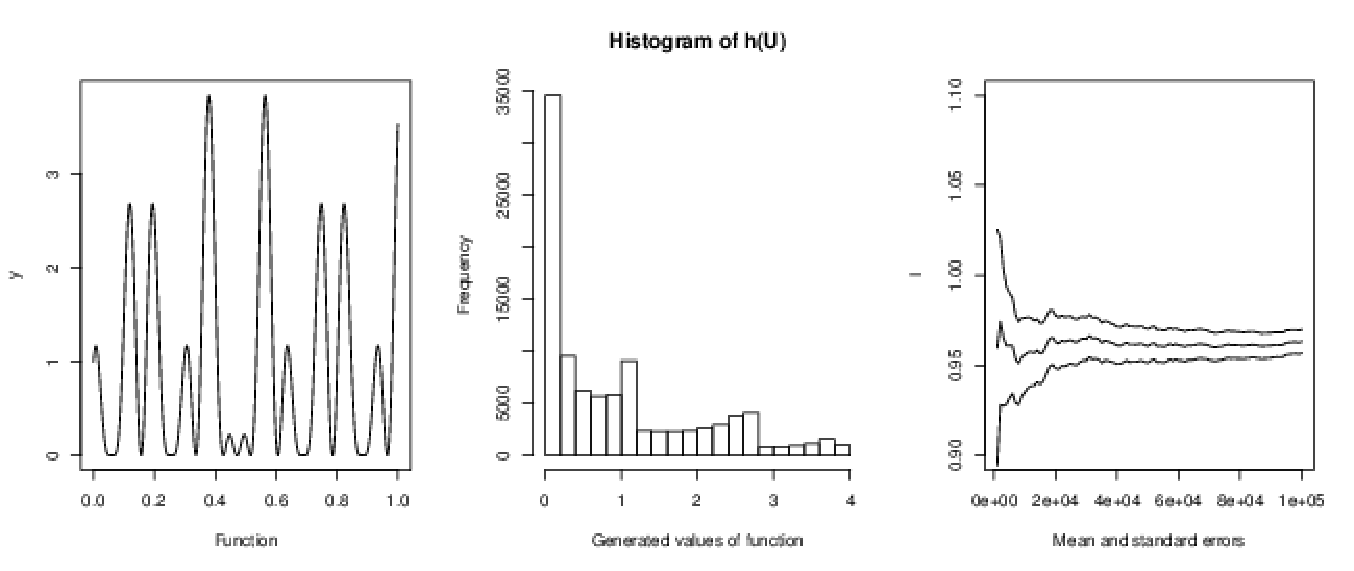
\includegraphics[scale=0.5]{MonteCarlo.pdf}



}



\frame{\frametitle{The general framework}\pause
\begin{equation}
R=\int f(x) dx \label{intI}
\end{equation}\pause
Let $g(x)$ be some density function that is easy to sample from. How
do we re-write (\ref{intI}) as the expectation of a function of a random
variable $X$ with density function $g(x)$?\pause
{\color{blank}\begin{equation}
R=\int \frac{f(x)}{g(x)} g(x) dx= \int h(x) g(x) dx,
\end{equation}
with $h(x)=\frac{f(x)}{g(x)}$.\pause}

So we now have $ R=E\{h(X)\}, $ where $X$ has the density function
$g(x)$. If we now sample $X_1,\ldots,X_n$ from $g(x)$, then evaluate
$h(X_1),\ldots,h(X_n)$, 
\begin{equation}
\hat{R}=\frac{1}{n}\sum_{i=1}^n h(X_i)
\end{equation}
is an unbiased estimator of $R$. }

\frame{\frametitle{Example 3} Use Monte Carlo integration to
estimate
\begin{equation}
R=\int_{-1}^1 \exp(-x^2)dx.
\end{equation}\pause
We'll consider two different choices for $g(x)$.
\begin{enumerate}
\item A uniform density on $[-1,1]$: $g(x)=0.5$ for $x\in [-1,1]$.\pause

We sample $X_1,\ldots,X_n$ from $U[-1,1]$, and estimate $R$ by
\begin{equation}
\hat{R}=\frac{1}{n}\sum_{i=1}^n
\frac{\exp(-X_i^2)}{g(X_i)}=\frac{1}{n}\sum_{i=1}^n2\exp(-X_i^2).
\end{equation}
\end{enumerate}
}

\frame{

\begin{enumerate}

\item[2] A normal density function $N(0,0.5)$.\pause

Note: sampled value $X$ from $g(x)$ not constrained to lie in
$[-1,1]$.\pause

 Re-write $R$ as
\begin{equation}
R=\int_{-\infty}^{\infty} I\{-1\le x \le 1\} \exp(-x^2)dx,
\end{equation}
where $I\{\}$ denotes the indicator function. \pause

We now sample $X_1,\ldots,X_n$ from $N(0,0.5)$ and estimate $R$ by
\begin{equation}
\hat{R}=\frac{1}{n}\sum_{i=1}^n \frac{I\{-1\le X_i \le
1\}\exp(-X_i^2)}{g(X_i)}=\frac{1}{n}\sum_{i=1}^n\pi^{1/2} I\{-1\le
X_i \le 1\}.
\end{equation}

\end{enumerate}\pause
\begin{block}{Key idea} $g(x)$ needs to mimic $f(x)$
as closely as possible. Consider again $ R=\int_{-1}^1\exp(-x^2)\rd x.
$\end{block}

}

\frame{

Two terrible choices of $g$:
\begin{enumerate}
\item A uniform density on $[0,1]$: $g(x)=1$ for $x \in [0,1]$.\pause
\begin{equation}
R=\int_{-\infty}^{\infty} I\{-1\le x \le 1\} \exp(-x^2)dx,
\end{equation}\pause
For $x \in [-1,0)$, we have $f(x)> 0 $ and $g(x)=0$. Must have
$g(x)>0$ for all $x$ where $f(x)>0$.\pause \item A normal density
$N(0,0.09)$.\pause

In this case, we have $g(x)>0$ for $x\in [-1,1]$, but we when we
sample $x$ from $g$, we expect around $95\%$ of the values to lie in
the range $(-0.6,6)$.

\pause The Monte Carlo estimate of $R$ is given by
\begin{equation}
\hat{R}=\frac{1}{n}\sum_{i=1}^n I\{-1\le X_i \le
1\}\frac{\exp(-X_i^2)\sqrt{0.18\pi}}{\exp(-5.56 X_i^2)}.
\end{equation}

\end{enumerate}
}



\frame{\frametitle{Convergence}\pause
\begin{itemize} \item Provided $f(x)>0 \Rightarrow
g(x)>0$, $\hat{R}$ will converge to $R$ as $n\rightarrow \infty$.
\pause\item Use the central limit theorem to derive a confidence
interval for $\hat{R}$:
\begin{equation}
\hat{R}\sim N\left(R,\frac{\sigma^2}{n}\right),
\end{equation}
where we estimate  $\sigma^2$ by
\begin{equation}
\hat{\sigma}^2=\frac{1}{n-1}\sum_{i=1}^n\left\{h(X_i)-\hat{R}\right\}^2
\end{equation}
\pause\item We can then report the confidence interval as
\begin{equation}
\hat{R} \pm Z_{1-\alpha/2}\sqrt{\hat{\sigma}^2/n},
\end{equation}
\pause\item Estimates of $\sigma^2$ in the example: $U[-1,1]:0.16$,
$N(0,0.5):0.42$, $N(0,0.09): 6.81$. \end{itemize}}

% \frame{\frametitle{Monte Carlo or numerical integration?}\pause
% \begin{itemize} \item
% Low dimensional integrals: numerical integration typically more
% efficient\pause\item  High dimensional integrals: Monte Carlo
% integration may be the only option. \pause \item Particularly
% suitable for integrals of the form
% \begin{equation}
% \int f(\bx)g(\bx)d\bx
% \end{equation}
% with $g(\bx)$ a density function of a random vector $\bX$, and
% $g(\bx)$ easy to sample from.
% \end{itemize}
% }



\frame{\frametitle{Comparison of Monte Carlo with numerical integration}
\framesubtitle{Mid-ordinate rule}
Consider finding $\ds{I=\int_0^1 f(x)~\rd x}$. There are many different numerical integration schemes we might use.

For example, the mid-ordinate rule is one of the simplest methods, and approximates $I$  by a sum
$$\quad \ds{\tilde{I}_{n}=\frac{1}{n} \sum_{i=1}^n f(x_i)},$$

The points $x_i=(i-\frac{1}{2})h$ are equally spaced at intervals of
$h=1/n$.

\begin{center}
%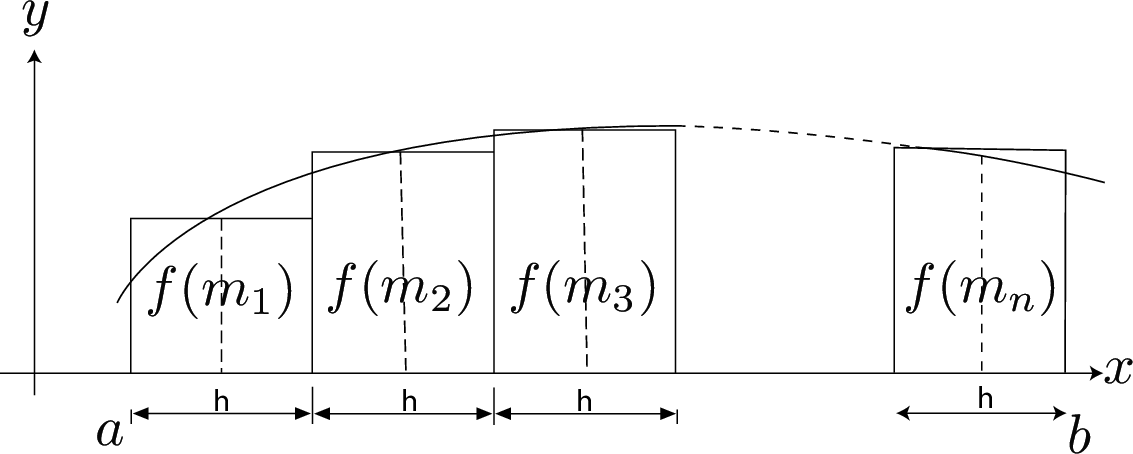
\includegraphics[scale=0.2]{midordinate}
\end{center}
}

\frame{\frametitle{Comparison of MC with numerical integration II}
\framesubtitle{Mid-ordinate rule error analysis}

For smooth 1-d functions the error rates for quadrature rules can be much better than Monte Carlo

\medskip
For example, if $f: [0,1] \rightarrow \mathbb{R}$ and $f''(x)$ is continuous, then
$$|I - \tilde{I}_n | \leq \frac{1}{24n^2} \max_{0\leq x\leq 1} |f''(x)|$$

So 
$$\mbox{RMSE}(\tilde{I}) = O(n^{-2})$$
i.e., it is a second order method\footnote{Other rules achieve higher errror rates. For example, Simpson's rule is a fourth order method.}
\pause

\medskip
This is much faster than Monte Carlo: to get an extra digit of accuracy we only need multiply $n$ by a factor of $\sqrt{10} =3.2$ 

}



\frame{\frametitle{Comparison of MC with numerical integration III}
\framesubtitle{Curse of dimensionality}
Classial quadrature methods work well for smooth 1d problems. But for $d$-dimensional integrals we have a problem. Suppose
$$I = \int_0^1\int_0^1\ldots \int_0^1 f(x_1, \ldots, x_d) {\rm d}x_1\ldots{\rm d}x_d$$

\pause
We can use the same $N$ point 1-d quadrature rules on each of the $d$ integrals. 

\medskip
This uses $n=N^d$ evaluations of $f$. The 1d mid-ordinate rule has error $O(N^{-2})$, so the d-dimensional mid-ordinate rule has error
$$|I-\tilde{I}| = O(N^{-2}) = O(n^{-2/d})$$
For $d=4$ this is the same as Monte Carlo. For larger $d$ it is worse.

\pause

In addition, we require $f$ to be smooth ($f''(x)$ to be continuous) for the method to work well.

\pause

Monte Carlo has the same $O(n^{-1/2})$ error rate regardless of $\dim(x)$ or $f''(x)$

}
\end{document}
